% -*- TeX:de -*-
\NeedsTeXFormat{LaTeX2e}
\documentclass[12pt,a4paper]{article}
\usepackage[german]{babel} % german text
\usepackage[DIV12]{typearea} % size of printable area
\usepackage[T1]{fontenc} % font encoding
%\usepackage[latin1]{inputenc} % most likely on Windows
\usepackage[utf8]{inputenc} % probably on Linux
\usepackage{multicol}

% PLOTTING
\usepackage{pgfplots} 
\usepackage{pgfplotstable}
\usepackage{url}
\usepackage{graphicx} % to include images
\usepackage{tikz}
\usepackage{subfigure} % for creating subfigures
\usepackage{amsmath} % a bunch of symbols
\usepackage{amssymb} % even more symbols
\usepackage{booktabs} % pretty tables
\usepackage{makecell} % multi row table heading

% a floating environment for circuits
\usepackage{float}
\usepackage{caption}

%\newfloat{circuit}{tbph}{circuits}
%\floatname{circuit}{Schaltplan}

% a floating environment for diagrams
%\newfloat{diagram}{tbph}{diagrams}
%\floatname{diagram}{Diagramm}

\selectlanguage{german} % use german

\begin{document}








%%%% TO DO
%
% - - Shorty:
%
% - - Tabelle "Messwerte Linsenbrennweite"
%		bitte bei jedem neuen e eine trennlinie... bin zu deppert ^^

% - - Patrick
%




%%%%%%% DECKBLATT %%%%%%%
\thispagestyle{empty}
			\begin{center}
			\Large{Fakultät für Physik}\\
			\end{center}
\begin{verbatim}


\end{verbatim}
							%Eintrag des Wintersemesters
			\begin{center}
			\textbf{\LARGE WS 2013/14}
			\end{center}
\begin{verbatim}


\end{verbatim}
			\begin{center}
			\textbf{\LARGE{Physikalisches Praktikum\\ für das Bachelorstudium}}
			\end{center}
\begin{verbatim}




\end{verbatim}

			\begin{center}
			\textbf{\LARGE{PROTOKOLL}}
			\end{center}
			
\begin{verbatim}





\end{verbatim}

			\begin{flushleft}
			\textbf{\Large{Experiment (Nr., Titel):}}\\
							%Experiment Nr. und Titel statt den Punkten eintragen
			\LARGE{PW8 Wellenoptik}	
			\end{flushleft}

\begin{verbatim}

\end{verbatim}	
							%Eintragen des Abgabedatums, oder des Erstelldatums des Protokolls
			\begin{flushleft}
			\textbf{\Large{Datum:}} \Large{21.11.2013}
			\end{flushleft}
			
\begin{verbatim}
\end{verbatim}
							%Namen der Protokollschreiber
		\begin{flushleft}
			\textbf{\Large{Namen:}} \Large{Patrick Braun, Johannes Kurz}
			\end{flushleft}

\begin{verbatim}


\end{verbatim}
							%Kurstag und Gruppennummer, zb. Fr/5
			\begin{flushleft}
			\textbf{\Large{Kurstag/Gruppe:}} \Large{DO/2}
			\end{flushleft}

\begin{verbatim}



\end{verbatim}
							%Name des Betreuers, das Praktikum betreute.
			\begin{flushleft}
			\LARGE{\textbf{Betreuer:}}	\Large{ Johanna Akbarzadeh }	
			\end{flushleft}

%%%%%%% DECKBLATT ENDE %%%%%%%
\pagebreak
\setlength{\columnsep}{20pt}
\begin{multicols}{2}


%\begin{figure}[H]
%	\centering
%	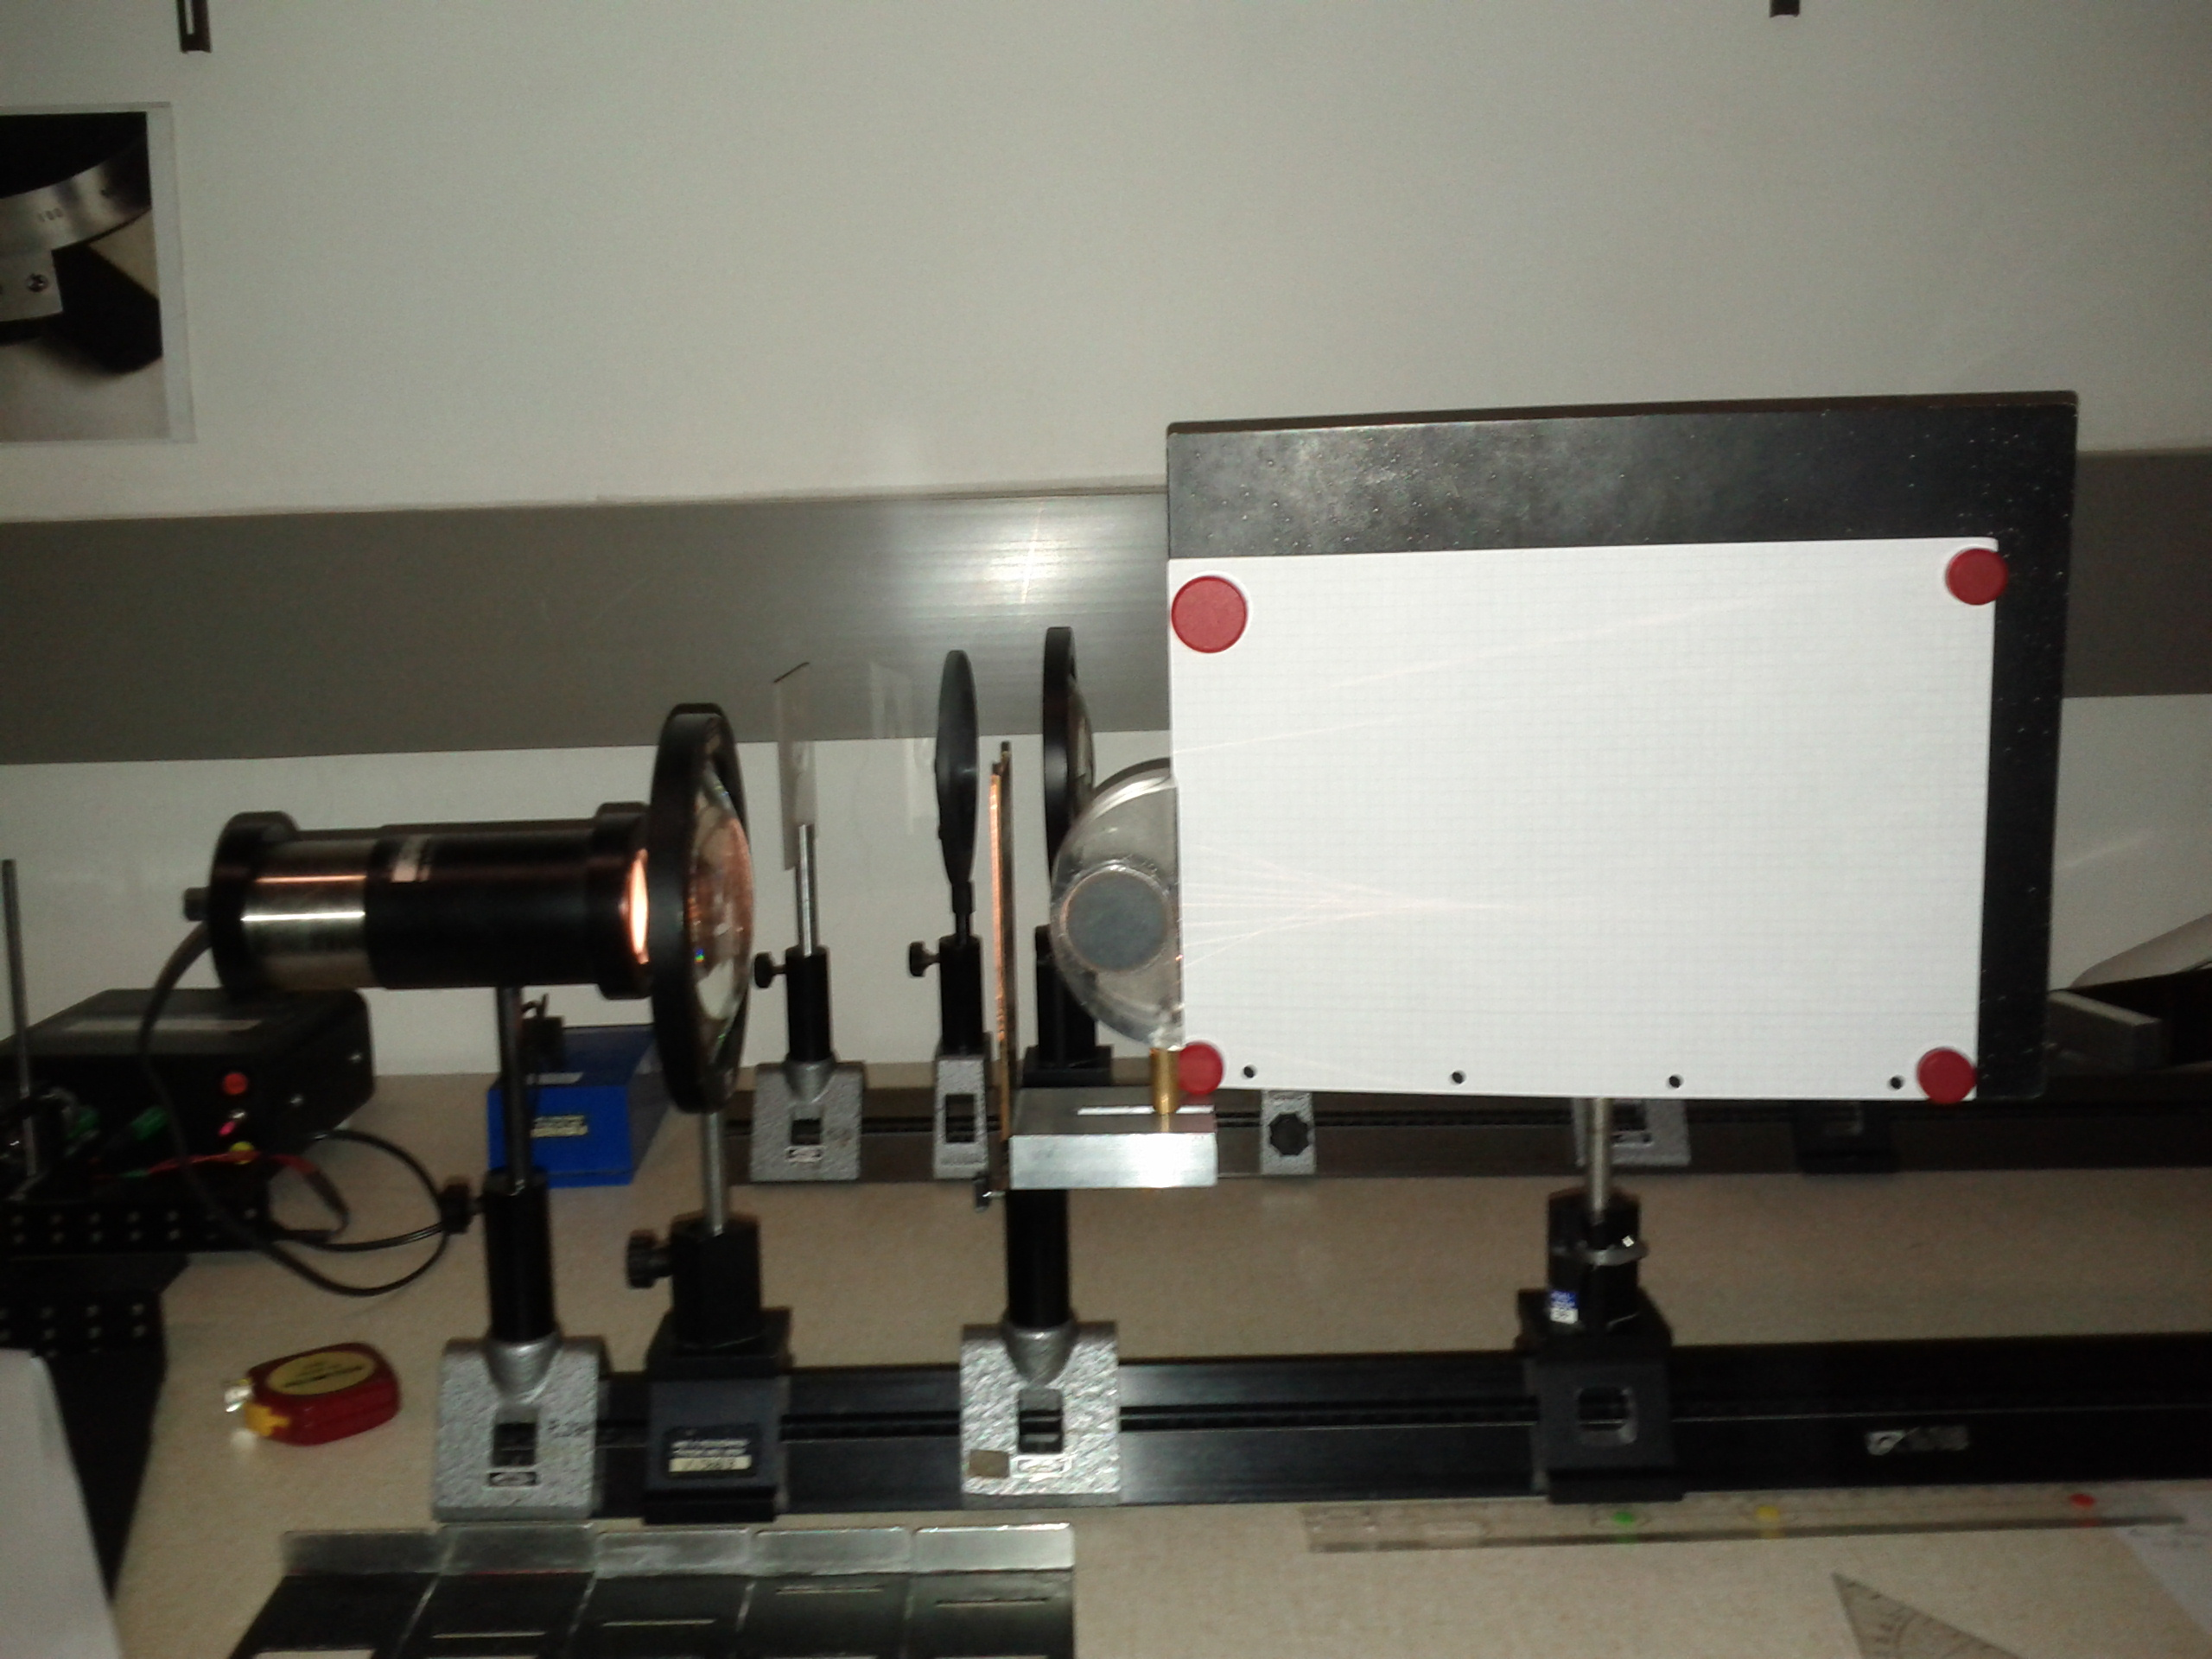
\includegraphics[scale=0.13]{./figure/linsenfehler.jpg}
%	\caption{Versuchaufbau Konvex-Plan Linse}
%	\label{fig:linsenfehler_aufbau}
%\end{figure}
%
%Glasprisma gegen Luft
%1.000292/sin(39grad28minutes)


%\begin{figure}[H]
%	\centering
%	\pgfplotstabletypeset[
%			columns={farbe, w,lambda},
%			col sep=&,
%			columns/farbe/.style={string type, column name=\makecell{$Farbe$\\} }, 
%			columns/w/.style={string type, column name=\makecell{$Winkel$\\$[Grad]$} }, 
%			columns/lambda/.style={column name=\makecell{$Wellenlänge$\\$[nm]$}, precision=0},
%			every head row/.style={before row=\hline,after row=\hline\hline},
%			every last row/.style={after row=\hline},
%			every first column/.style={column type/.add={|}{} },
%			every last column/.style={column type/.add={}{|} }
%			]{
%			farbe & w & lambda
%			rot & 47$^\circ$ 39' & 543
%			grün & 48$^\circ$ 58' & 508
%			zyan & 49$^\circ$ 29' & 479
%			blau & 49$^\circ$ 45' & 467
%			violett & 50$^\circ$ 18' & 441
%			
%			}
%	\caption{Farben, Winkel und Wellenlängen der Cadmium-Dampflampe}
%	\label{fig:werte_cadmiumdampflampe}
%\end{figure}



%%%%%%%%%%%%%%%%%%%%%%%%%%%%%%%%%%%%%%%%%%%%%%%%
\end{multicols}
\begin{figure}[H]
	\centering
	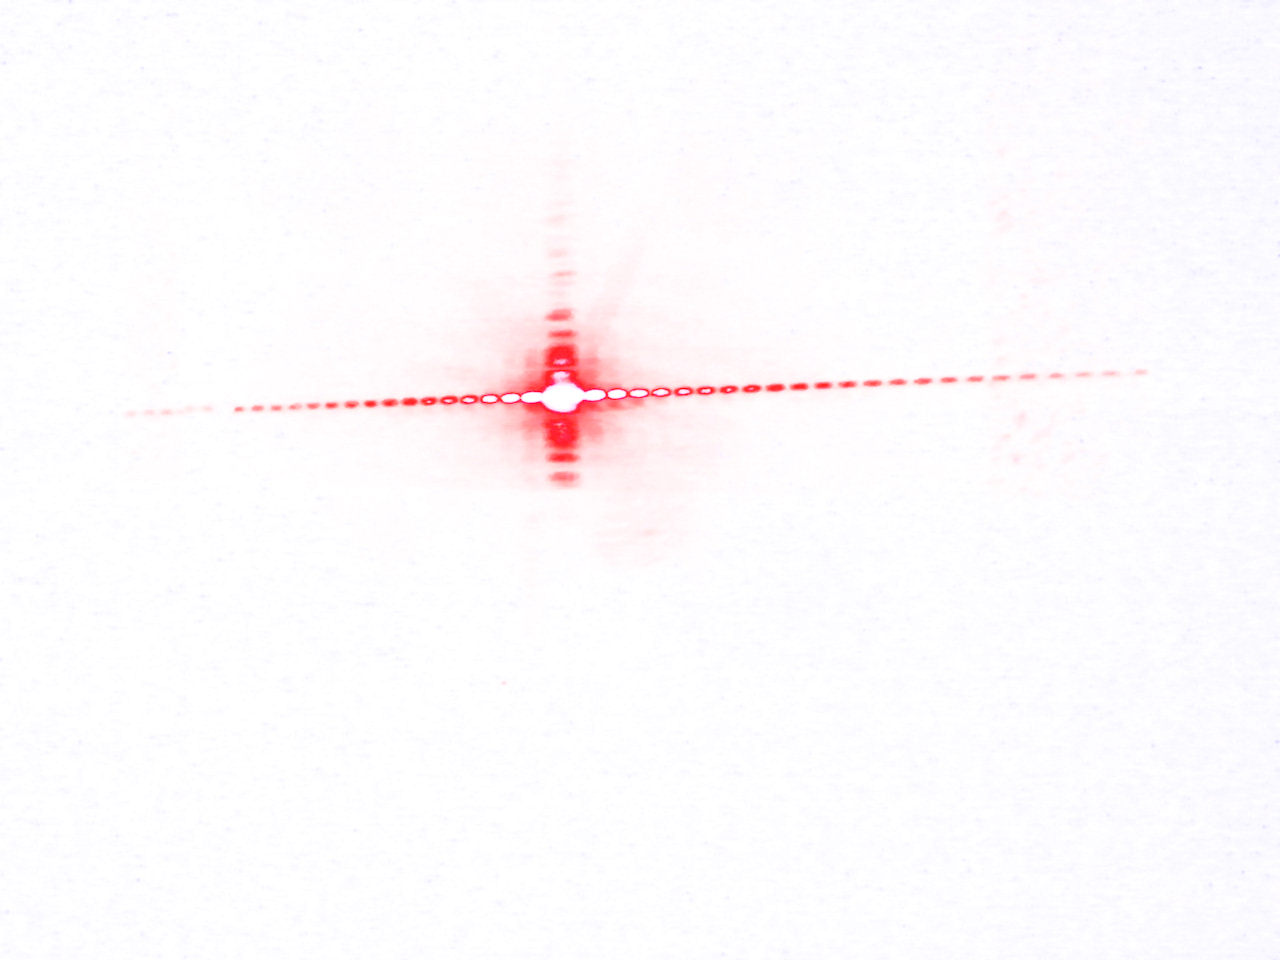
\includegraphics[scale=0.35]{./figure/beugung.png}
	\caption{Beugungsmuster Einzelspalt (echtes Foto; schwarz durch weiß ersetzt)}
	\label{fig:beugungsmuster}
\end{figure}

\begin{multicols}{2}

\section{Beugung am Spalt und Doppelspalt}
Im ersten Experiment sollen ein Einzelspalt und ein Doppelspalt über die Beugung von monochromatischem Licht untersucht werden. Die Lichtquelle ist ein roter Laser (Wellenlänge $\lambda = 632.8nm$). \\
Die Ausbreitung von Licht kann beschrieben werden durch Kugelwellen an jedem Punkt (Huygens-Fresnel-Prinzip). Fällt das Licht auf den Spalt (oder auch den Doppelspalt oder ein Gitter), ergeben sich Gangunterschiede durch die Begrenzungen. Dadurch ergibt sich ein (hier rotes) Beugungsmuster auf dem Schirm (Abb. \ref{fig:beugungsmuster}). 
\\
Durch die Vermessung des Abstandes vom Einzelspalt zum Schirm (Abb. \ref{fig:messwerte_einzelspalt}) und dem Abstand zwischen den Minima kann auf den Beugungswinkel (für jedes Minimum) geschlossen werden, und daraus direkt die Spaltbreite ermittelt werden [1](Glg. 13):
$$a = \frac{n*\lambda}{sin(\alpha_{min,n})} $$
$$\alpha_n = arctan(\frac{b_n}{R})$$
a...Spaltbreite\\
$b_n$...Abstand zwischen Minimum und 0-ter Ordnung\\
R...Abstand vom Spalt zum Schirm\\
$\lambda$...Wellenlänge des verwendeten Lichtes\\
\\
Beim Doppelspalt ergibt sich ein ähnliches Beugungsmuster, mit dem Unterschied, dass der zentrale helle Punkt mehrere Minima und Maxima enthält. Diese entstehen durch Interferenz der Wellen aus beiden Spalten.\\
Der Spaltabstand $d$ und die Spaltbreite $a$ ergeben in ihrem Verhältnis die Ausprägung der Interferenz. So kann (durch zählen der Interferenz-Minima und Bestimmung der Spaltbreite,wie im Einzelspalt) der Spaltabstand bestimmt werden.
$$ a = \frac{\lambda * n}{\alpha_n} $$
und
$$\frac{d}{a} = x$$
\noindent
x... Minima in eine Richtung im zentralen Beugungsmaximum\\
d... Spaltabstand (Mitte zu Mitte)\\
\\
Die Winkelmessung erfolgt wie beim Einzelspalt.
In beiden Fällen wird eine Fernfeldbeugung beobachtet (die Wellen sind näherungsweise eben). Konkret muss der Abstand zum Beobachtungsschirm R folgender Gleichung genügen:
$$R \textgreater \frac{a^2}{\lambda}$$
\\
%d/a = x\\
%wobei: a = lambda*n/alpha_n (wellenlänge mal ordnung / gemessener winkel der jeweiligen ordnung)\\
%
%alpha_n = atan(messung/(2*R)) weil wir ja eine länge gemessen haben, in entfernung R... der faktor 1/2 kommt, weilma immer beide seiten gemessen und halbiert haben
%11 maxima -> x = 6

\subsection{Messwerte und Ergebnisse}



\end{multicols}
\begin{figure}[H]
	\centering
	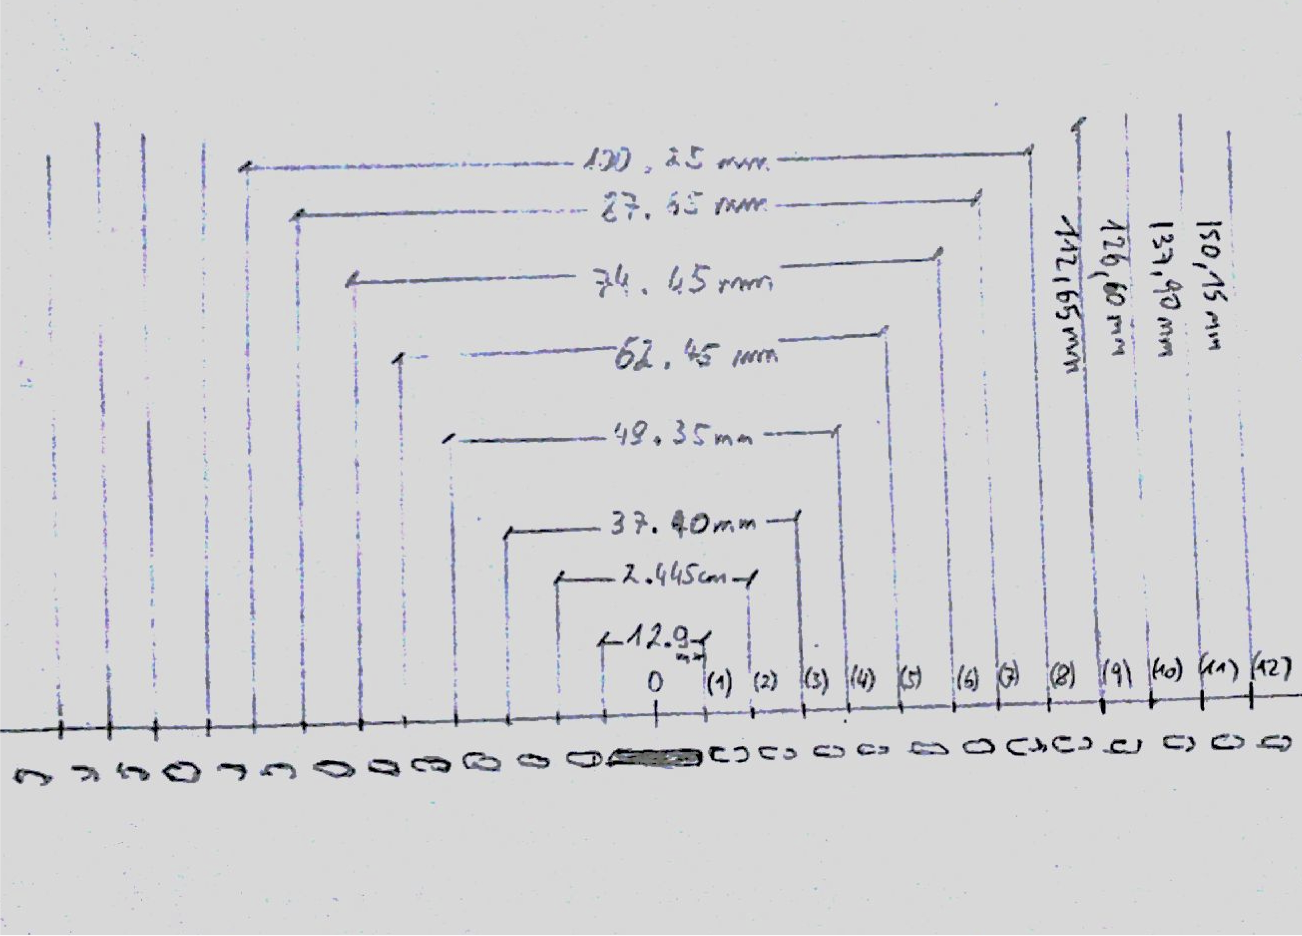
\includegraphics[scale=0.9]{./figure/einzelspalt_beugung.png}
	\caption{Beugungsmuster Einzelspalt mit Werten}
	\label{fig:messwerte_einzelspalt}
\end{figure}
\begin{figure}[H]
	\centering
	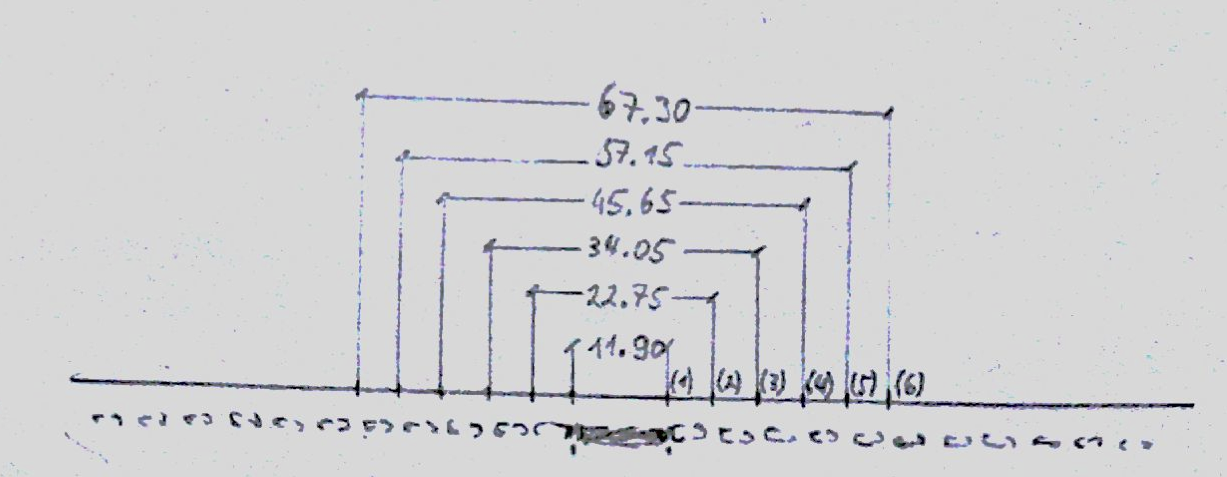
\includegraphics[scale=0.9]{./figure/doppelspalt_beugung.png}
	\caption{Beugungsmuster Doppelspalt mit Werten; ohne Minima und Maxima in der 0-ten Ordnung}
	\label{fig:messwerte_doppelspalt}
\end{figure}

\begin{multicols}{2}
\noindent
Wellenlänge des Laser der bei Einzel- und Doppelspalt verwendet wurde:
$$\lambda = 632.8nm$$

\noindent \textbf{Einzelspalt}\\
Aus den Messwerten aus \ref{tab:werte_einzelspalt} wurde in QTI-Plot eine Lineare Regression durchgeführt (Abbildung \ref{fig:einzelspalt_linreg}). 
\begin{figure}[H]
	\centering
	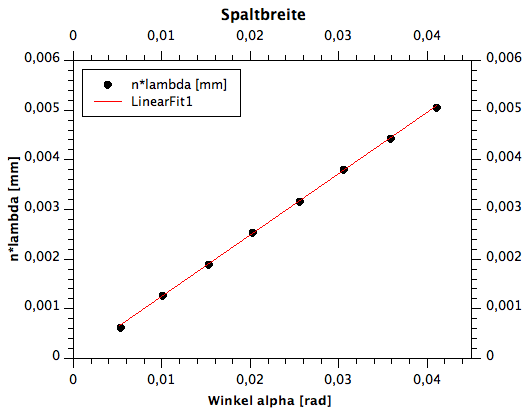
\includegraphics[scale=0.40]{./figure/linreg_einzelspalt.png}
	\caption{Lineare Regression Einzelspalt}
	\label{fig:einzelspalt_linreg}
\end{figure}
Daraus ergibt sich eine Spaltbreite von 
$$a = (0.1234 \pm 0.0065)mm$$
\begin{figure}[H]
	\centering
	\pgfplotstabletypeset[
			columns={abstand, n},
			col sep=&,
			columns/abstand/.style={precision=2, zerofill, column name=\makecell{$Abstand$\\$(\pm 0.05)[mm]$} }, 
			columns/n/.style={column name=\makecell{$n$\\$(Ordnung)$}, precision=0},
			every head row/.style={before row=\hline,after row=\hline\hline},
			every last row/.style={after row=\hline},
			every first column/.style={column type/.add={|}{} },
			every last column/.style={column type/.add={}{|} }
			]{
			abstand & n
			12.9 & 1
			24.45 & 2
			37.40 & 3
			49.35& 4
			62.45 & 5
			74.45 & 6
			87.45 & 7
			100.25 & 8
			
			}
	\caption{Messwerte Einzelspalt}
	\label{tab:werte_einzelspalt}
\end{figure}

\noindent
\textbf{Doppelspalt}\\
Es konnten \textbf{11 Maxima} in der 0-ten Ordnung gezählt werden, was zu \textbf{x = 6} führt. 
Mit den Messwerten aus \ref{tab:werte_doppelspalt} wurde in QTI-Plot eine Lineare Regression durchgeführt (Abbildung \ref{fig:doppelspalt_linreg}). 
Außerdem musste der Abstand $R$ (Spalt-Schirm) gemessen werden um den Winkel zu berechnen:
$$R = (108.1 \pm 0.2)cm$$
Die Steigung ergibt folgende Spaltbreite:
$$a = (0.122 \pm 0.001)mm$$
\begin{figure}[H]
	\centering
	\pgfplotstabletypeset[
			columns={abstand, n},
			col sep=&,
			columns/abstand/.style={precision=2, zerofill, column name=\makecell{$Abstand$\\$(\pm 0.05)[mm]$} }, 
			columns/n/.style={column name=\makecell{$n$\\$(Ordnung)$}, precision=0},
			every head row/.style={before row=\hline,after row=\hline\hline},
			every last row/.style={after row=\hline},
			every first column/.style={column type/.add={|}{} },
			every last column/.style={column type/.add={}{|} }
			]{
			abstand & n
			11.9 & 1
			22.75 & 2
			34.05 & 3
			45.65& 4
			57.15 & 5
			67.30 & 6
			}
	\caption{Messwerte Doppelspalt}
	\label{tab:werte_doppelspalt}
\end{figure}
\begin{figure}[H]
	\centering
	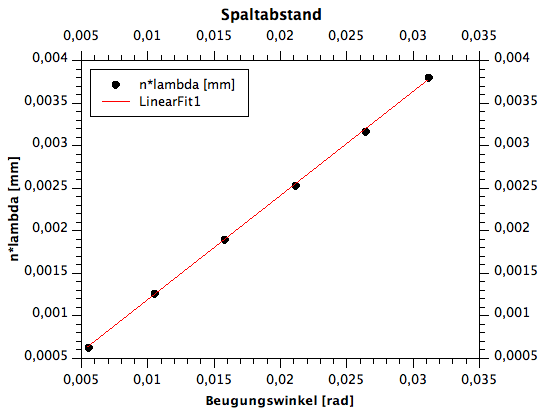
\includegraphics[scale=0.4]{./figure/linreg_doppelspalt.png}
	\caption{Lineare Regression Doppelspalt}
	\label{fig:doppelspalt_linreg}
\end{figure}
\noindent
Der Spaltabstand $d$ ergibt sich durch:
$$\frac{d}{a} = x$$
\noindent
\\
$$d = 6\cdot 0.122 = (0.732 \pm 0.001)mm$$

\subsection{Diskussion}
Die Ausrichtung des Lasers auf den Spalt gestaltet sich etwas wackelig in diesem Aufbau, da der Laser per Hand gedreht wurde. Ein und ausschalten verstellt ihn leicht. Nachdem aber alle Messungen pro Spalt in einem Durchgang durchgeführt wurden, entsteht hierbei kein Fehler.\\
Die Messunsicherheiten durch Schublehre und Maßband konnten klein abgeschätzt werden (ihre Auflösungen), was, nach den linearen Fits, zu guten Ergebnissen geführt hat.\\
%Beim Doppelspalt war eine genaue Einstellung des Lasers nur bei absoluter Dunkelheit und gleichzeitiger Beobachtung der 0-ten Ordnung erfolgreich, da bei einer kleinen Abweichung bereits die Minima und Maxima verschwimmen. Trotz guter Justierung konnten bei den ersten Zählungen nur 9 statt 11 Maxima gesehen werden.  


%%%%%%%%%%%%%%%%%%%%%%%%%%%%%%%%%%%%%%%%%%%%%%%%
\section{Wellenlängenmessung am Gitter}

Nachdem im 1. Versuch also die Beugungserscheinungen von Licht am Einzel- und am Doppelspalt
untersucht wurden, geht es in diesem Teil von PW8 um die Beugung am Gitter.\\
Jeder einzelne Spalt des Gitters erzeugt seine Einzelspaltbeugung, wobei Inteferenzen durch die Wellen aus all den anderen Spalten entstehen, ähnlich wie beim Doppelspalt. Im Unterschied zu diesem inteferieren nach dem Gitter jedoch Wellen aus einer sehr großen Zahl von Einzelspalten.
Daraus resultiert ein Beugungsbild von sehr schmalen, stark ausgeprägten Maxima mit sehr kleinen, praktisch dunklen, Gebieten dazwischen.\\
Durch die Beugung von Lichtstrahlen an einem Gitter soll das Spektrum einer Lampe bestimmt werden:\\
Die untersuchte Lampe strahlt nur einige bestimmte Wellenlängen ab. Da die Beugung von der Wellenlänge abhängt, werden die verschiedenen Farben unterschiedlich stark gebeugt. Durch die engen und deutlichen Beugungsmaxima, die vom Gitter verursacht werden, lassen sich die Beugungswinkel der einzelnen Farben bestimmen und ihre Wellenlänge berechnen:
$$\lambda = \sin{\alpha_{max,n}}\cdot \frac{b}{n}$$
wobei $b$ (beim Doppelspalt der Abstand zwischen beiden Spalten) hier der Gitterkonstante $g=10 \mu m$ entspricht.\\
Zur Messung der jeweiligen Winkel wird mit einem Kollimatorrohr ein Parallelstrahlenbündel durch das Gitter geschickt und die verschiedenen Beugungsmaxima mit einem Fernrohr auf einem Goniometer anvisiert.\\
%reference auf die zeichnung%
Zuerst wird die Nulllage des Systems durch Zielen auf das zentrale Maximum ermittelt. In diesem sind alle Farben der Lampe vereint, daher ist es (annähernd) weiß.\\
Es werden 3 Beugungen, jeweils links und rechts des zentralen Maximums, von insgesamt 3 Spektralfarben auf diese Art vermessen (siehe Abb. \ref{fig:beugungeswinkel_quecksilberspektrum}). Aus allen gemessenen Beugungswinkel werden die entsprechenden Wellenlängen berechnet. Die Bildung des Mittelwertes ergibt schließlich die Wellenlänge der jeweiligen Farbe sodass, im Vergleich mit den Literaturwerten verschiedener Lampen, ermittelt werden kann, um welche Spektrallampe es sich handelt.

\subsection{Messwerte und Ergebnisse}

\begin{figure}[H]
	\centering
	\pgfplotstabletypeset[
			columns={ordnung, gruen, gelb, blau},
			col sep=&,
			columns/ordnung/.style={string type, column name=\makecell{$Ordnung$\\Maximum} }, 
			columns/gruen/.style={string type, column name=\makecell{$gruen$\\$[Grad]$\\$\pm 2'$} }, 
			columns/gelb/.style={string type, column name=\makecell{$gelb$\\$[Grad]$\\$\pm 2'$}, precision=0},
			columns/blau/.style={string type, column name=\makecell{$blau$\\$[Grad]$\\$\pm 2'$}, precision=0},
			every head row/.style={before row=\hline,after row=\hline\hline},
			every last row/.style={after row=\hline},
			every first column/.style={column type/.add={|}{} },
			every last column/.style={column type/.add={}{|} }
			]{
			ordnung & gruen & gelb & blau
			links 1: & 3$^\circ$ 8' & 3$^\circ$ 19' & 2$^\circ$ 27'
			rechts 1: & 3$^\circ$ 9' & 3$^\circ$ 21' & 2$^\circ$ 32'
			links 2: & 6$^\circ$ 17' & 6$^\circ$ 38' & 4$^\circ$ 57'
			rechts 2: & 6$^\circ$ 18' & 6$^\circ$ 39' & 5$^\circ$ 7'
			links 3: & 9$^\circ$ 26' &  &
			rechts 3: & 9$^\circ$ 27' &  &
			links 4: & & 13$^\circ$ 26' & 10$^\circ$ 0'
			rechts 4: & & 13$^\circ$ 24' & 10$^\circ$ 7'
			
			
			
						
			}
	\caption{Beugungswinkel 3er Spektralfarben, je 6 Messungen}
	\label{fig:beugungeswinkel_quecksilberspektrum}
\end{figure}


Gitterkonstante $g= 10 \mu m$

$$gruen: \lambda_{gruen}=(547.60 \pm 0.76)nm$$
$$gelb: \lambda_{gelb}=(579.9 \pm 1.5)nm$$
$$blau: \lambda_{blau}=(436.7 \pm 4.3)nm$$\\



\noindent \textbf{Quecksilberdampflampe:}\\
Wellenlängen (Literaturwert [2]):\\
$gruen: \lambda_{gruen}=546.07nm$\\
$gelb: \lambda_{gelb}=579.07nm$\\
$blau: \lambda_{blau}=435.83nm$\\

\subsection{Diskussion}
Jeder der 3 Wellenlängen wurde durch ein Mittel aus 6 berechneten Einzelwerten ermittelt. 
Die angegebene Unsicherheit ist der Standarderror of the mean mit student-t-Korrektur.\\
\\
Alle 3 gemessenen Spektralfarben weisen Wellenlängen auf, die sehr nah am Literaturwert liegen. Einzig  für die Farbe grün liegt dieser außerhalb des gemessenen Unsicherheitsbereiches.\\
Der jedoch ist von allen 3 Farben der engste und dürfte daher etwas zu klein abgeschätzt worden sein. Die Streuung der Messwerte für grün ist vergleichsweise gering, was sich in einem kleineren Standarderror niederschlägt, als dem der anderen beiden Farben. Die ursprüngliche Messunsicherheit wurde für alle 3 Farben gleich gewählt mit $0^\circ \pm 2'$.\\
\\
Da die Werte so gering streuen, und die Ergebnisse der anderen beiden Farben gut am erwarteten Wert liegen, ist es wahrscheinlich, dass ein leichter systematischer Fehler vorliegt.\\
Auffällig ist, dass die Ergebnisse für die Wellenlängen  auf der rechten Seite tendenziell eher zu hoch, auf der linken eher zu niedrig sind. Das deutet stark darauf hin, dass die Nulllage zu ungenau bestimmt wurde.\\
Es konnten jedoch durch neue Berechnungen mit verschobener Nullage keine Ergebnisse erzielt werden, die näher am Literaturwert liegen und die Werte der anderen beiden Farben nicht kompromittieren. Die Tendenz nach rechts ist zwar zu erkennen, dürfte aber nicht ausschlaggebend sein, oder gerade nur so, um den Wert für grün, dank seiner geringen Streuung, leicht zu verrücken.\\
Andere Ursachen, wie fehlerhafte Messungen (grün war die erste Messreihe) sind nicht auszuschließen.\\
Um dieser Abweichung auf den Grund zu gehen, müsste der Versuch also wiederholt werden.\\
\\
Da die vorliegenden Ergebnisse jedoch klar ausreichen, um das Emissionsspektrum aus den vorgeschlagenen Möglichkeiten eindeutig als Quecksilberdampflampe zu identifizieren, sind die Messung und die berechneten Werte jedenfalls genau genug, um die gestellte Frage zu klären.

%%%%%%%%%%%%%%%%%%%%%%%%%%%%%%%%%%%%%%%%%%%%%%%%
\section{Newtonsche Ringe}

Die Newtonringe sind ein Inteferenzbild von Licht, dass durch eine sehr schwach gekrümmte plan-konvexe Linse fällt, an die direkt eine Glasplatte anschließt. Zwischen Platte und Linse ist also, abgesehen vom Berührungspunkt, ein kurzer Abschnitt Luft, der, dank der schwachen Krümmung der Linse, nahezu ein rechtwinkeliges Dreieck bildet (siehe Abb. \ref{fig:newtonringe_reflexion}).\\


\begin{figure}[H]
	\centering
	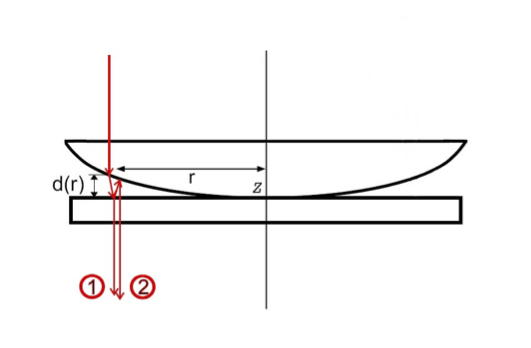
\includegraphics[scale=0.80]{./figure/newtonringe_strahlengang.png}
	\caption{Strahlengang in Transmission}
	\label{fig:newtonringe_transmission}
\end{figure}


Durch den Unterschied im Brechungsindex, zwischen Glas und Luft und durch teilweise Reflexion, werden aus jedem einfallenden Strahl eine Vielzahl (nahezu) paralleler Strahlen mit leicht unterschiedlichen Phasen. Aus der Überlagerung der Erzeugnisse aller einfallender Strahlen ergeben sich schließlich die beobachtbaren Newtonringe, ein Inteferenzmuster.\\
Das gleiche Prinzip gilt auch für die Strahlen, die reflektiert werden und durch die Linse wieder austreten. Auch hier entstehen fast-parallele Strahlen mit Phasenunterschieden.\\
Um den Effekt schön zu erzielen, ist Licht mit ausreichend großer Kohärenzlänge nötig. In diesem Versuch wird eine Halogenlampe verwendet.
\\
Das Licht aus der Lampe fällt auf das System aus Linse und Glasplatte. Unter Verwendung 2er Strahlteiler und Sammellinsen werden sowohl die Newtonringe in Reflexion, als auch die in Transmission, direkt nebeneinander auf einen Schirm projiziert (Abb. \ref{fig:newtonringe_aufbau}).

\begin{figure}[H]
	\centering
	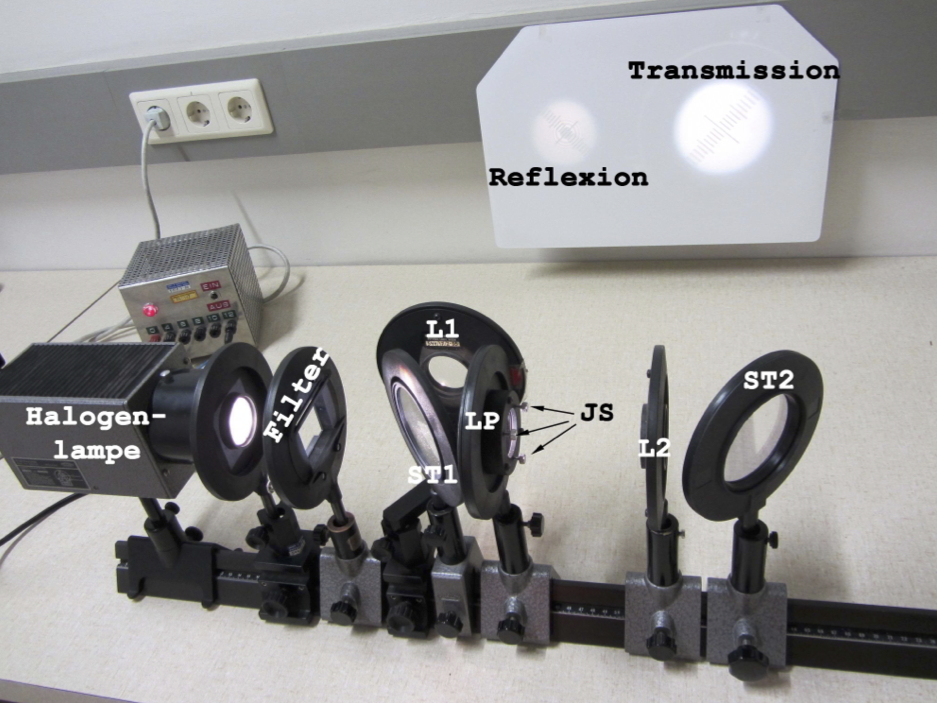
\includegraphics[scale=0.45]{./figure/newtonringe_aufbau.png}
	\caption{Versuchsaufbau - Newtonringe}
	\label{fig:newtonringe_aufbau}
\end{figure}

\noindent $Strahlteiler: ST1, ST2$\\
$Sammellinsen: L1, L2$\\
$Linse-Glasplatte: LP$\\
\\
Wird der Versuchsaufbau ohne Farbfilter eingeschaltet, lassen sich die Newtonringe zwar gut als solche erkennen, jedoch nicht eindeutig begrenzen. Die verschiedenen Spektralfarben werden unterschiedlich stark "abgelenkt": Die unterschiedlichen Wellenlängen bewirken, dass die Phasenverschiebungen verschiedene Minima und Maxima für verschiedene Spektralfarben erzeugen. Dadurch verschmieren die Ringe.\\
Je weiter außen sie betrachtet werden, desto unschärfer wird das Bild.\\
Durch den Farbfilter wird eine Wellenlänge herausgegriffen. Das verringert die Intensität deutlich, führt jedoch zu einer sehr viel klareren Abgrenzung der einzelnen Ringe voneinander.\\
der hier verwendete Farbfilter:\\
grün: $\lambda = (518 \pm 3) nm$\\
\\
Aus geometrischen Betrachtungen ergibt sich für den Zusammenhang zwischen dem Radius $r$ der Newtonringe und dem Krümmungsradius $R$ der Linse:
$$r^2 = (2R-d)d$$
$d$... Abstand zwischen Linse und Platte\\
Auslöschung liegt im reflektierten Fall vor, wenn:
$$2d_k + \frac{\lambda}{2}=(2k+1)(\frac{\lambda}{2})$$
Da $R$ sehr viel größer ist als $d$ gilt also für Auslöschungen im Reflexionsfall:
$$r_k^2 =kR\lambda$$
konstruktive Interferenz:
$$r_k^2=(2k+1R \frac{\lambda}{2})$$
Im Fall der Ringe in Transmission gelten beide Gleichungen für die jeweils andere Art von Interferenz.\\
\\
Der Krümmungsradius $R$ soll bestimmt werden, indem die Radien $r_k$ verschiedener Maxima bzw. Minima in beiden Interferenzbildern gemessen werden um so R in linearer Regression zu ermitteln:
$$R=\frac{r_k^2}{k \lambda}$$

\noindent Die Inteferenzringe werden auf ein Blatt Papier projiziert, markiert und anschließend mit einer Schublehre vermessen.
Dazu ist außerdem auf der Glasplatte des Systems ein mm-Maßstab angebracht, der es erlaubt, die Größenverhältnisse der Abbildung zu bestimmen.

\subsection{Messwerte und Ergebnisse}

Umrechnungsfaktor Reflexion: $\frac{5}{18}$\\
\indent $18mm_{Messung} = 5mm_{wirklich}$\\
Transmission: $\frac{1}{5}$\\
\indent $25mm_{Messung} = 5mm_{wirklich}$\\
\\
Wellenlänge: $\lambda = (518\pm 3)nm$

\begin{figure}[H]
	\centering
	\pgfplotstabletypeset[
			columns={reflex, transmiss},
			col sep=&,
			columns/reflex/.style={column name=\makecell{Radius $r_k$\\Reflexion\\$[mm]$\\ $\pm 0.1mm$} }, 
			columns/transmiss/.style={column name=\makecell{Radius $r_k$\\Transmission\\ $[mm]$\\ $\pm 0.1mm$}}, 
			every head row/.style={before row=\hline,after row=\hline\hline},
			every last row/.style={after row=\hline},
			every first column/.style={column type/.add={|}{} },
			every last column/.style={column type/.add={}{|} }
			]{
			reflex & transmiss
			%6.2 & 
%			10.5 & 13.6
%			14.3 & 19.4
%			17.0 & 23.1
%			19.8 & 26.1
%			22.2 & 29.4
%			24.1 & 32.0
			
			1.7 & 2.7
			2.9 & 3.9
			4.0 & 4.6
			4.7 & 5.2
			5.6 & 5.9
			6.2& 6.4
			6.7 & 			
			
			
			}
	\caption{gemessene Radien der Newtonringe}
	\label{fig:radien_newtonringe}
\end{figure}



\end{multicols}
\begin{figure}[H]
	\centering
	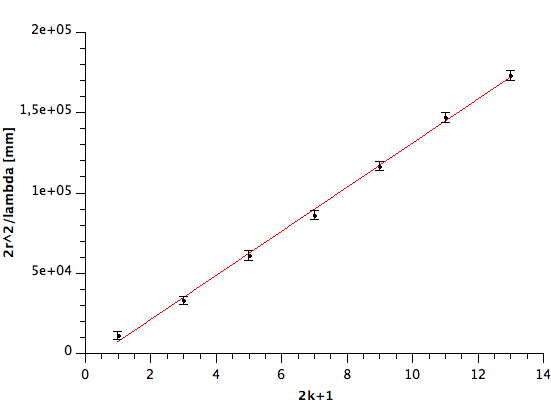
\includegraphics[scale=0.70]{./figure/newtonringe_reflex_regress.png}
	\caption{Newtonringe - Reflexion: $R=2r_k^2*\frac{1}{\lambda (2k+1)}$}
	\label{fig:newtonringe_reflex_regress}
\end{figure}

%Aus der Steigung: R der Linse
$$R_{Reflexion} = 13.73 \pm 0.27)m$$



\begin{figure}[H]
	\centering
	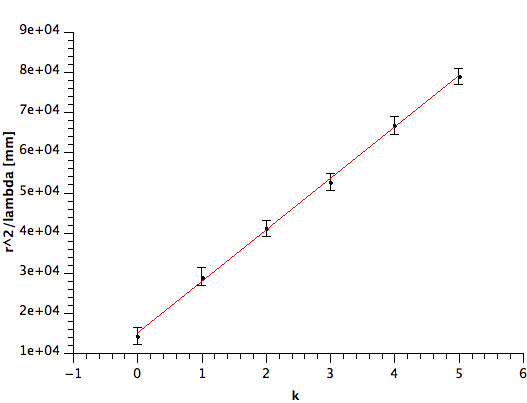
\includegraphics[scale=0.70]{./figure/newtonringe_transmiss_regress.png}
	\caption{Newtonringe - Transmission: $R=r_k^2\frac{1}{\lambda *k}$}
	\label{fig:newtonringe_transmiss_regress}
\end{figure}

$$R_{Transmission}=(12.82 \pm 0.87)m$$

%B (y-intercept) = 1,509918148328588e+04 +/- 2,520381237651498e+03
%A (slope) = 1,281922284232692e+04 +/- 8,668173766933726e+02
\begin{multicols}{2}

\subsection{Diskussion}

Der Krümmungsradius $R$ aus den Messungen der Reflexions-Newtonringe stimmt sehr genau mit den Angaben der Betreuerin überein (etwa 13.7 m). Die Abweichung der einzelnen Messpunkte von der Regressionsgerade ist klein und auch die einzelnen Unsicherheiten auf der y-Achse konnten klein abgeschätzt werden (Abb. \ref{fig:newtonringe_reflex_regress}).
\\
(Die Unsicherheit von $\lambda$ ist vorgegeben, die der gemessenen Radien mit dem doppelten der Auflösung der Schublehre -$\pm 0.1 mm$ -  vorsichtig gewählt)
\\
\\
Die Messung der aus den Transmissions-Ringen ist etwas problematischer:\\
Zwar liegt das Ergebnis durchaus in der Nähe des erwarteten Wertes, die einzelnen Messwerte schwanken jedoch deutlich, im Vergleich zur anderen Messung. Das führt zu einer fast 4mal größeren Unsicherheit (Abb. \ref{fig:newtonringe_transmiss_regress}).\\
Schon das Markieren der Ringe am Papier hat erwarten lassen, dass diese Messung ungenauer ist. Die hellen Ringe aus der Transmission waren deutlich schwieriger zu erkennen und weniger eindeutig.\\
Teil der Aufgabenstellung ist die Frage nach dem Kontrast zwischen hellen und dunklen Ringen, der im transmittierten Inteferenzbild schwächer sein soll, als im reflektierten:\\
Da weniger Licht an einer Grenzfläche reflektiert wird, als durchgeht, ist der Kontrast im Transmissionsfall (2 Reflexionen, siehe Abb. \ref{fig:newtonringe_transmission}) viele geringer, als im Reflexionsfall (nur 1 Reflexion).\\
Dieser Effekt hat zur Schwierigkeit der Messung wesentlich beigetragen, und erklärt, zumindest teilweise, das ungenauere Ergebnis im Transmissionsfall.\\
\\
Die Vergrößerung der transmittierten Abbildung ist leicht größer, was zu einer Verkleinerung der Messunsicherheit führt. Die ist jedoch klein gegen die Ungenauigkeiten durch weniger Intensität und unklare Ringgrenzen.\\
\\
Der Versuch ließe sich vielleicht durch eine stärkere Lampe noch genauer durchführen. Umständlicher aber auch effektiv wäre womöglich ein vertikaler Aufbau, um die Markierung flach auf dem Tisch durchführen zu können oder zumindest eine stabile Wand als Schirm zu verwenden.\\
Die erzielten Ergebnisse sind jedoch gut am erwarteten Wert.

\section{Quellen}
$[1]$ Leitfaden, \url{http://www.univie.ac.at/anfpra/neu1/pw/pw8/PW8.pdf}\\
$[2]$ Quecksilberdampflampe, \url{http://de.wikipedia.org/wiki/Quecksilberdampflampe}\\
%$[2]$

\end{multicols}

\begin{figure}[H]
	\centering
	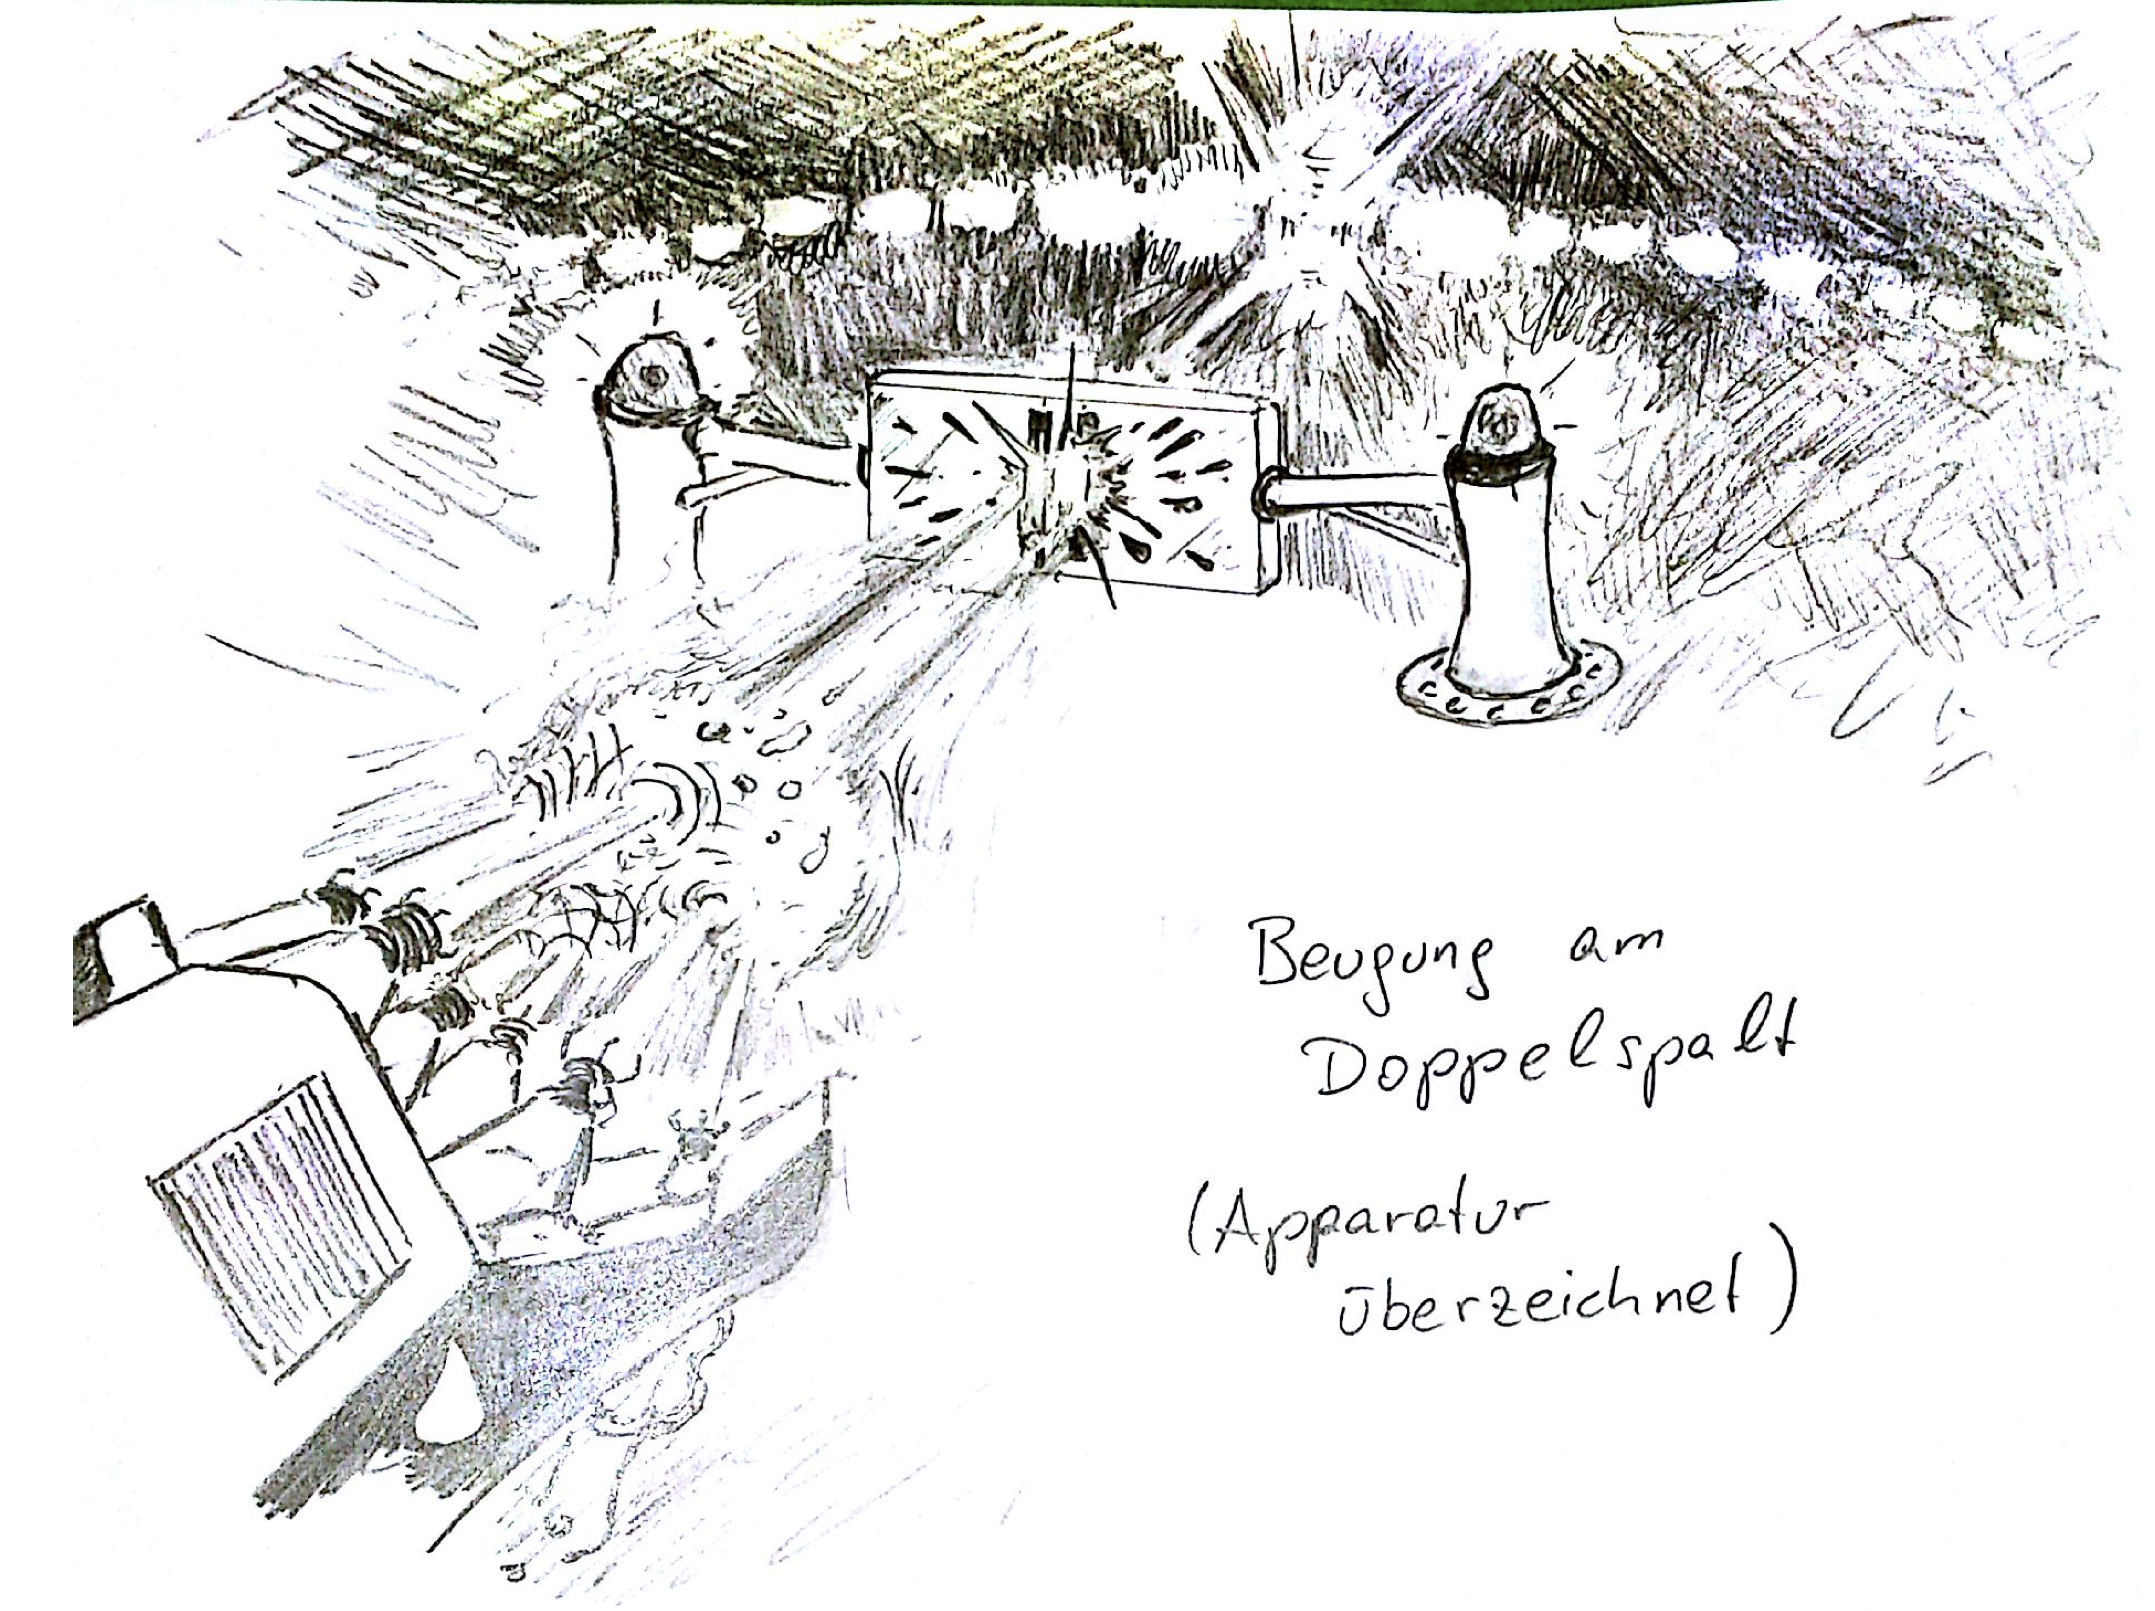
\includegraphics[scale=0.60]{./figure/laser_kanone.png}
	\caption{Beugung am Doppelspalt}
	\label{fig:laser_kanone}
\end{figure}

\end{document}